\newpage
\section{Here's the Pitch}


The steepness of a roof is called its \textit{slope}
or \textit{pitch}. This is a fraction where the numerator is
the \textit{rise} of the roof and the denominator is
the \textit{run}. The denominator is usually $12$. Hence a slope of
\[
\frac{7}{12}
\]
says that the roof goes up $7''$ for every $12''$. Note there are several
other notations for pitch. The one we are presenting here is not only
rather common, it is also mathematically correct!

\begin{prob}
Here is a diagram of a roof: 
\[
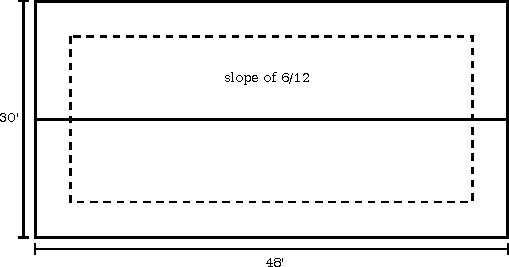
\includegraphics{../graphics/pitch1.pdf}
\]
Find the area of the roof. 
\end{prob}

\begin{prob}
Here is a diagram of a roof with different slopes for each side: 
\[
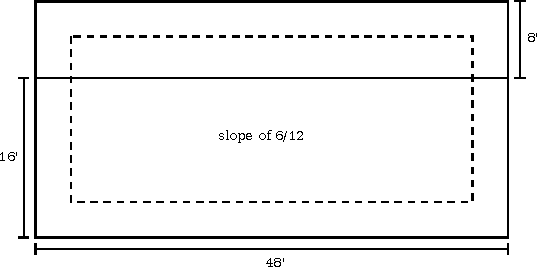
\includegraphics{../graphics/pitch2.pdf}
\]
First find the missing slope, then find the area of the roof.
\end{prob}

\begin{prob}
Here is a diagram of a roof: 
\[
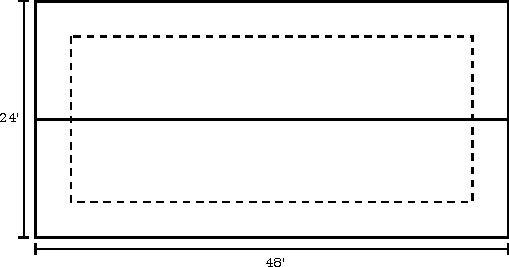
\includegraphics{../graphics/pitch3.pdf}
\]
The area of the roof is 1248 square feet. Find the slope of the
roof.
\end{prob}

\begin{prob}
Here is a diagram of a roof: 
\[
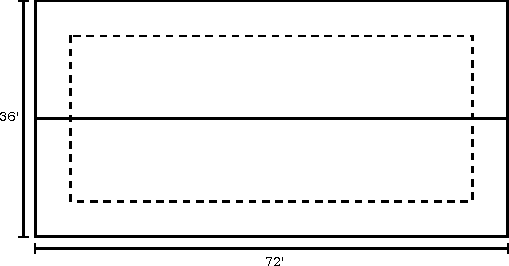
\includegraphics{../graphics/pitch4.pdf}
\]
The area of the roof is 2808 square feet. Find the slope of the
roof.
\end{prob}


\begin{prob}
Explain how to measure the slope of a roof using two rulers and a
level. Give examples of measurements that you could take, and say what
the pitch would be in each case.
\end{prob}

\break

\begin{prob}
In Europe, it is more common to measure the steepness of a roof using
the angle of the roof from horizontal. For example, a roof whose
slope is $12/12$ has an angle of $45^\circ$. Complete the conversion table below:
\[
{\renewcommand{\arraystretch}{1.5}
\begin{array}{c|c}
\text{slope} & \text{angle} \\ \hline\hline
1/12 &  \\ \hline
2/12 &  \\ \hline
3/12 &  \\ \hline
4/12 &  \\ \hline
5/12 &  \\ \hline
6/12 &  \\ \hline
7/12 &  \\ \hline
8/12 &  \\ \hline
9/12 &  \\ \hline
10/12 &  \\ \hline
11/12 &  \\ \hline
12/12 & 
\end{array}}
\]
Hint: You'll need to remember something from a previous course.
\end{prob}


